\section{Pathing}
To my knowledge, a method of path planning across a decentralized system we have defined does not exist. Similar work has been done for centralized systems in \cite{FTC-A} and \cite{CTF-A}. Therefore, we propose a modification to standard A*. As we don't have another method to compare against, we will use a greedy euclidean-based search as comparison. Since our system is intended to coordinate with other cameras within it, we are assuming that a camera in the upper layer has knowledge of other cameras' positions relative to itself. If this were not the case, we would be required to perform a blind search such as Uniform Cost Search. These cameras do not share any other knowledge.

\subsection{Greedy}
For the greedy method of path planning, we only take into account the euclidean distance between the current camera and the goal camera. Therefore nothing at the child level of the graph is considered. At each camera, we take the neighbor with the lowest euclidean distance to the goal camera and set it as the current camera. This would be equivalent to traversing a path through a camera in the direction of the goal, and replanning at each camera. This method runs until the goal is found. The path is rebuilt as described in Algorithm \ref{Rebuild_Path}

\subsection{A*}
I present two version of A* to solve the problem of decentralized pathing through this system. There are two primary changes made to the standard A* algorithm which are used in both versions. These changes are given in Algorithm \ref{D-A*_Cost} and \ref{Rebuild_Path}. Changes more specific to the two versions of D-A* will be presented in their section. 

\begin{algorithm}[h]
\caption{D-A* Cost}
\label{D-A*_Cost}
\begin{algorithmic}[1]
\REQUIRE \ \\
Current Camera, $C_C$ \\
Neighbor Camera, $C_N$ \\
\IF{$C_C$ is \textit{this}}
	\STATE Let $P_O$ represent a point in the overlap region between $C_C$ and $C_N$
	\RETURN path\_cost($C_C$.startPoint, $P_O$)
\ELSE
	\RETURN $C_C$.request\_cost($C_C$, $C_N$)
\ENDIF
\end{algorithmic}
\end{algorithm}

\begin{algorithm}[h]
\caption{Rebuild Path}
\label{Rebuild_Path}
\begin{algorithmic}[1]
\REQUIRE \ \\
Goal Camera, $C_G$ \\
Goal Point, $P_G$ in $C_G$ 
\STATE Let $C$ = $C_G$
\STATE Let $P_F$ be an initially empty set of edges representing the final path
\STATE Let $P_T$ be an initially empty set of edges representing an intermediate path
\WHILE{$C$.parent $\neq$ NULL}
	\STATE $P_T$ = \textit{this}.requestPath($C$.startPoint, $C$.endPoint)
	\STATE $P_T$.append($P_F$)
	\STATE $P_F$ = $P_T$
	\STATE $P_T$.clear()
\ENDWHILE
\end{algorithmic}
\end{algorithm}
\subsubsection{D-A* V1}
I propose Decentralized A* (D-A*), a modified version of A* to plan a path across a set of decentralized, connected parent nodes. The children of these nodes will be taken into account during the planning process. Work in decentralized path planning has been done in \cite{DecentralizedPlanningVelagapudi}, \cite{DeadlockDraganjac}. However, these algorithms run in a decentralized system where a robot or set of robots are self-sufficient. In this environment, I have a set of parent nodes creating a path through their children which the robots will follow. As it is decentralized, each parent node will have no knowledge of the internals of its neighbors. Therefore it will be necessary to use some form of network communication to request necessary information from other parent nodes.

This algorithm will follow a top down pathing approach. The majority of the pathing will happen on the parent layer with information such as cost coming from the child layer of the requested camera. The cost will be the shortest path across the child layer from the starting edge of the current camera to a point in the overlap region of the neighboring camera. For this algorithm, it is assumed that a pathing algorithm to determine the shortest paths on the child layer of every camera has already run. The primary difference between this and standard A* is the cost function and path rebuilding. This algorithm runs solely on the source camera which forces communication with other cameras for information. The path will be entirely rebuilt on the source camera, and passed along to the robot. Given all of this, I propose the following modifications to standard cost, path reconstruction, and A* algorithms in algorithms \ref{D-A*_Cost}, \ref{Rebuild_Path}, and \ref{D-A*} respectively. 

As this is a decentralized system, all method calls will be done on the source camera. Any calls that obtain information from a different camera will require a request to that camera. 

Per Algorithm \ref{D-A*_Cost}, if the source node is not the node we are seeking cost for, it will request cost from $C_C$ for a path from the start point of $C_C$ to a point in the overlap region shared with the neighbor in question. The cost of the path currently consists only of the length. Ideally, this could be expanded to include congestion at a time \(t\)

After the goal is found, the path will be rebuilt starting from the goal camera as described in Algorithm \ref{Rebuild_Path}. The source camera will request the path between the start and end points from the goal camera, and append it to the final path. The interior of the loop concatenates the most recently requested path onto the front of the final path. 

%Since we are operating on a standard grid, the currently used heuristic is Eucledian distance. However, as this is a modification to standard A*, the heuristic can be changed to fit the situation. 

The final modification to A* is on line 15 in algorithm \ref{D-A*}. As the cost in this implementation depends on the parent node, we check the cost of the path to reach the goal. Assume a goal camera, $C_G$ has two neighbors, $N_1$ and $N_2$. If $cost(N_1, C_G) < cost(N_2, C_G)$, then A* will assign $N_1$ as the parent of $C_G$.  Assume $O_{P1}$ is the overlap point between neighbor 1 and the goal. Assume $O_{P2}$ is the overlap point between neighbor 2 and the goal. Due to cost being directionally dependent, this could cause a problem when finding the path from the start point of $C_G$ to the goal point. This is because it is possible that $$pathCost(O_{P2}, goalPoint) < pathCost(O_{P1}, goalPoint)$$ If the difference is large enough, it may be true that the cost required to get to to the goal point would be lower if we followed the path along $N_2$.
\begin{align*}
	cost(N_1, C_G) &+ pathCost(O_{P1}, C_G.endpoint) \\
	&> \\
	cost(N_2, C_G) &+ pathCost(O_{P2}, C_G.endpoint)
\end{align*}
This would mean the path going through $N_1$ is suboptimal. Therefore we must take the extra path cost into account when assigning a parent to the goal node. This issue extends in that it could happen to any node farther than two steps from $C_S$. This causes A* to rarely produce a path which is longer than the path produced by greedy. In the case of the goal node, it is easily solvable. In the case of a random node, I believe this problem is not worth solving as it becomes very complex. I will discuss this in more detail in Sections 4.3 and 6.1.2.


\begin{algorithm}
\caption{D-A*}
\label{D-A*}
\begin{algorithmic}[1]
\REQUIRE \ \\
Start Camera, $C_s$ \\
Goal Camera, $C_g$ \\
Start Point $P_s$ in $C_s$
\STATE add $C_s$ to \textit{openSet}
\WHILE{\textit{openSet} is not empty}
	\STATE \textit{$N_C$} = \textit{openSet.pop}
	\IF{\textit{$N_C$} is $C_g$}
		\RETURN $C_S$.rebuild\_path()
	\ENDIF
	\FOR{each \textit{neighbor} of \textit{$N_C$}}
		\IF{\textit{neighbor} in \textit{closedSet}}
			\STATE \textbf{continue}
		\ENDIF
		\IF{\textit{neighbor} not in \textit{openSet}}
			\STATE add \textit{neighbor} to \textit{openSet}
		\ENDIF
		\STATE \textit{potentialCost} $=$ \textit{$N_C$}.costSoFar + $C_S$.cost(\textit{$N_C$, neighbor})
		\IF{\textit{neighbor} is $C_G$}
			\STATE \textit{ov\_point} $=$ find\_overlap\_point($N_C$, $C_g$
			\STATE \textit{potentialCost} $=$ $C_S$.getPathCost($C_G$.startPoint, $C_G$.endPoint)
		\ENDIF
		\IF{\textit{potential\_cost} $<$ \textit{neighbor}.costSoFar}
			\STATE $N_C$.endPoint $=$ find\_overlap\_point($N_C$, neighbor)
			\STATE \textit{neighbor}.startPoint = $N_C$.endPoint
			\STATE \textit{neighbor}.parent $=$ \textit{$N_C$}
			\STATE \textit{neighbor}.costSoFar $=$ \textit{potentialCost}
			\STATE \textit{neighbor}.costToEnd $\leftarrow$ \textit{neighbor}.costSoFar + heuristic()
		\ENDIF		 
	\ENDFOR
	\STATE \textit{closedSet}.add(\textit{$N_C$})
	\STATE \textit{openSet}.remove(\textit{$N_C$})
\ENDWHILE
\RETURN failure
\end{algorithmic}
\end{algorithm}
\subsubsection{D-A* V2}
This version of D-A* is modified such that the number of requests made on the network will be reduced. In the first version, only one set of information is gained per request. Assume a source node $C_S$ and a node currently being expanded, $C_C$. Since all processing is done in $C_S$, any time information is required from $C_C$, a request must be made. Due to the way A* works, only one neighbor of $C_C$ is processed at a time. Therefore, as we need information, such as cost, about each neighbor of $C_C$, a request must be made for each neighbor. As at least one neighbor of $C_C$ has already been discovered and expanded at this point, we have a maximum of 3 requests made to the same node. 

The goal of this version of D-A* is to reduce the number of requests made to $C_C$ by doing all neighbor processing on $C_C$ and returning the gathered information back to $C_S$. This gives us a maximum of 1 request to $C_C$ as illustrated in Figure \ref{fig:ReqDiagrams}. As these requests are only part of the total requests made, we will not achieve a 66\% decrease in total requests.

To do this, the calculations and evaluations for each neighbor must be moved into a function separate from D-A*. By moving lines 14-25 of Algorithm \ref{D-A*} into a separate function, \textit{getNeighborInfo()}, we can make a request on $C_C$ to run this function and return the information back. Given that, I propose the required modification to the neighbor loop in Algorithm \ref{V2Neighbor}. The evaluation of which set owns the neighbor is still required to be outside \textit{getNeighborInfo()} as we only want information on neighbors outside the closed set.

This modification was successful in greatly reducing the number of requests made across the network. This will be discussed more in the results section. 

\begin{algorithm}
\caption{D-A* V2 Neighbor Loop}
\label{V2Neighbor}
\begin{algorithmic}[1]
\STATE let \textit{neighbors} be an initially empty list
\FOR{each \textit{neighbor} of \textit{$N_C$}}
	\IF{\textit{neighbor} in \textit{closedSet}}
		\STATE \textbf{continue}
	\ENDIF
	\IF{\textit{neighbor} not in \textit{openSet}}
		\STATE add \textit{neighbor} to \textit{openSet}
	\ENDIF
	\STATE add \textit{neighbor} to \textit{neighbors}
\ENDFOR		 
\STATE $C_S$.getNeighborInfo(\textit{neighbors}, $N_C$, $C_G$)
\end{algorithmic}
\end{algorithm}

\begin{figure}[h]
\centering
\begin{subfigure}{.49\textwidth}
\centering
	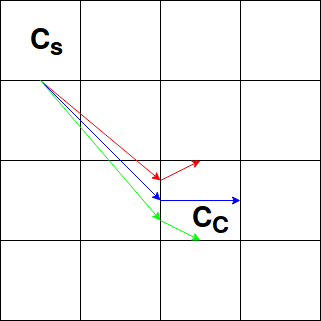
\includegraphics[width=.4\linewidth]{RequestDiagramV1}
	\caption{V1}
	\label{fig:v1Req}
\end{subfigure}
\begin{subfigure}{.49\textwidth}
	\centering
	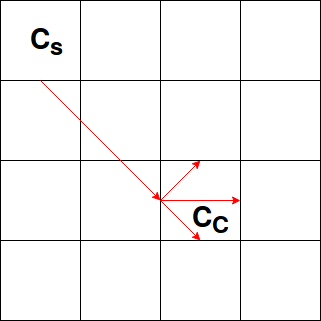
\includegraphics[width=.4\linewidth]{RequestDiagramV2}
	\caption{V2}
	\label{fig:v2Req}
\end{subfigure}
\caption{A visual representation of $C_S$ requesting information on $C_C$'s neighbors using D-A* V1 (a) and V2 (b). Each arrow from $C_S$ to $C_C$ represents a request on $C_C$ followed by which neighbor the request gathers information from.}
\label{fig:ReqDiagrams}
\end{figure}
\subsection{Lookahead Problem}
As described in section 4.2.1, pathing through this system is directionally dependant. This leads to issues in that the chosen path may not be the true optimal path. Because of this, a greedy search will outperform A* 2.42\% of the time. In this section, I will explain why this happens, but the percentage will be explained in results. 

This problem can be solved using a different representation of the system graph. However, without using a different representation, I believe it is not feasibly solvable. 

The graph representation used in this work is not a true representation of the graph. In this work, the graph is being represented as a grid of NxN nodes. The problem with this representation is that it assumes we are pathing from node center to node center, whereas we're actually pathing from node edge to node edge. Therefore, a more true representation would require treating each edge of each ceiling camera as a node or set of nodes as shown in Figure \ref{fig:RepDiagrams}. Using this representation would allow correct handling of directional dependency such that A* always outperforms greedy. However, this also means the potential size of the queue will be much larger, requiring more memory, and A* would take much longer to run.

\begin{figure}[h]
\centering
\begin{subfigure}{.49\textwidth}
\centering
	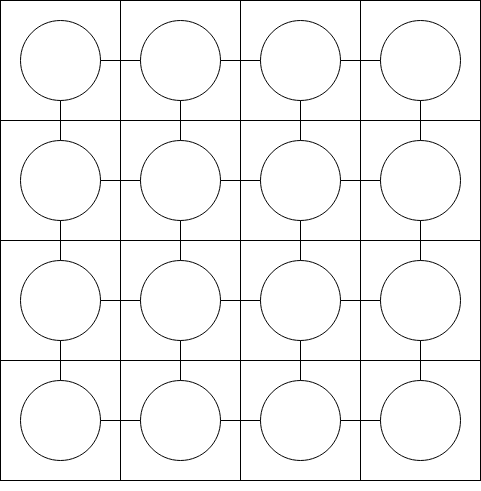
\includegraphics[width=.4\linewidth]{CurrentRepresentation}
	\caption{Current Representation}
	\label{fig:CurRep}
\end{subfigure}
\begin{subfigure}{.49\textwidth}
	\centering
	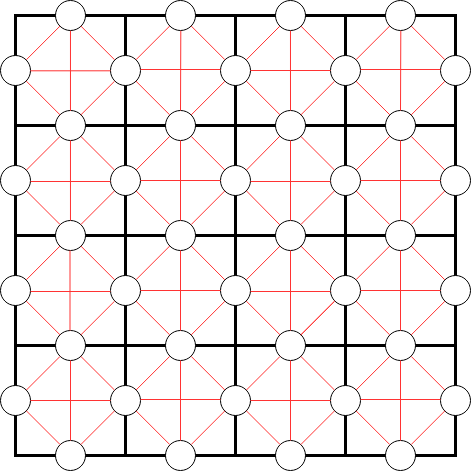
\includegraphics[width=.4\linewidth]{TrueRepresentation}
	\caption{"True" Representation}
	\label{fig:TrueRep}
\end{subfigure}
\caption{The currently used reprsentation (a) and the "True" representation (b). Note that both representations assume all nodes in the parent layer are connected to their neighbors. (b) assumes each edge can be reached by every other edge and that there is only one overlap point per edge.}
\label{fig:RepDiagrams}
\end{figure}

Using the current representation, the worst case Space Complexity is $\mathcal{O}(N^2)$. In the true representation, there are $N+1$ sets of $N$ nodes both from top to bottom and left to right of the grid. This gives us a worst case of $\mathcal{O}(2(N^2 + N))$. While this is technically equivalent to the current representation, this system is setup using cameras with limited memory. Since it is practically more than double the amount of memory, this could pose a problem in a low memory system.

The time complexity is equivalent for the two representations, $\mathcal{O}(|V| + |E|)$. While the equation hasn't changed, the values for $V$ and $E$ have. As described above, $V$ is now $2(N^2 + N)$. Per \cite{HPA}, a grid has four corner nodes, $4N-8$ edge nodes, and $(N-2)^2$ middle nodes. Using the assumption that each node in the grid is connected to all immediate neighbors, corner nodes have two edges, edge nodes have three edges, and middle nodes have four edges. The total edge count for the current representation is 

$$2(4) + 3(4N-8) + 4(N-2)^2$$

This gives a total edge count of $4N(N-1)$. As each edge is counted twice with this equation, the final edge total is actually $2N(N-1)$ for the current representation. In the true representation, the worst case is a path from any edge to any other edge within the same region. With M edge points per region and NxN regions, the edge total is $\frac{M(M-1)}{2}N^2 \geq 2N(N-1)$ for all values $N \geq 2$ and $M \geq 1$. In practice, this is always true as a graph with one parent node or one edge point is pointless for this system.

This representation of the system would increase the optimality of paths through it.  Whether or not it is worth using is dependent on what is more critical to the system in its specific environment: more optimal paths or reduced runtime and memory usage.

In the current representation, the reason A* is outperformed is a combination of being unable to feasibly look ahead far enough, and greedy getting lucky. As previously explained, the pathing in this system is directionally dependent. This means that if a robot enters a region from the top, it has to continue its path from the top. Therefore it is possible that the path from a different overlap point to the next neighbor is significantly shorter than the path the robot is forced to take. 

Assume we are pathing through a region $N_R$. Also assume that the cost to go to $N_R$ through $N_A$ is lower than the cost through $N_B$. In this case, A* will elect to take the path through $N_A$. By doing this, it will no longer recognize $N_B$ as a potential parent to $N_R$, and will therefore not see any paths in $N_R$ originating from $O_{N_B, N_R}$. Therein lies the problem. Assume we path to a node $N_C$ from $N_R$. It is possible that while the the cost through $N_B$ was higher than $N_A$, the cost from $O_{N_A, N_R}$ to $O_{N_R, N_C}$ is significantly higher than $O_{N_B, N_R}$ to $O_{N_R, N_C}$. If the difference is significant enough, it may be true that $$cost(N_A, N_R) + cost(O_{N_A, N_R}, O_{N_R, N_C}) > cost(N_B, N_R) + cost(O_{N_B, N_R}, O_{N_R, N_C})$$

If this is true, the path found will be suboptimal. In this same case, it is possible that greedy happens to choose $N_B$ rather than $N_A$ as the predecessor to $N_R$. If this happens, greedy will return a lower cost path than A*.

Ideally, this problem could be solved by looking ahead. Basically, check the cost of $O_{N_B, N_R}$ to $O_{N_R, N_C}$ and $O_{N_A, N_R}$ to $O_{N_R, N_C}$, and consider them when determining who the parent should be. There are a couple issues with this idea. First, just because the step we lookahead changes the decision at this stage doesn't mean it's going to be beneficial long term. In the previous example, a path to $N_C$ was made regardless of whether or not $N_A$ or $N_B$ was used. It's entirely possible that pathing through $N_A$ would've led to a different neighbor of $N_R$, $N_D$, due to being lower cost than $N_C$. If it is still high enough that the path through $N_B$ is optimal up to that point, this lookahead method would choose $N_B$. However, it is possible that the path after reaching $N_D$ is much shorter than the path after reaching $N_C$. In this case, the lookahead would choose a suboptimal path. Adding more stages to the lookahead does not fix the problem unless it can look ahead to the goal. At this point, it'd be the same as calculating multiple paths. The second issue with the lookahead method is that it assumes we know which region we are going to next. To get around this, one may think to use the minimum cost path in the next stage as a heuristic. It would be admissible as it underestimates distance. However, it will not work as it falls back to the first reason in that it cannot see multiple steps into the future. 

I have attempted to visualize this explanation in Figure \ref{LookaheadRef} with path cost in terms of $c$. Assume the path from $N_D$ to the goal is $c$ and the path from $N_C$ to the goal is $2c$.


With all of that, I believe that solving this problem without changing representations is, at the very least, impractical. 

\begin{figure}
\centering
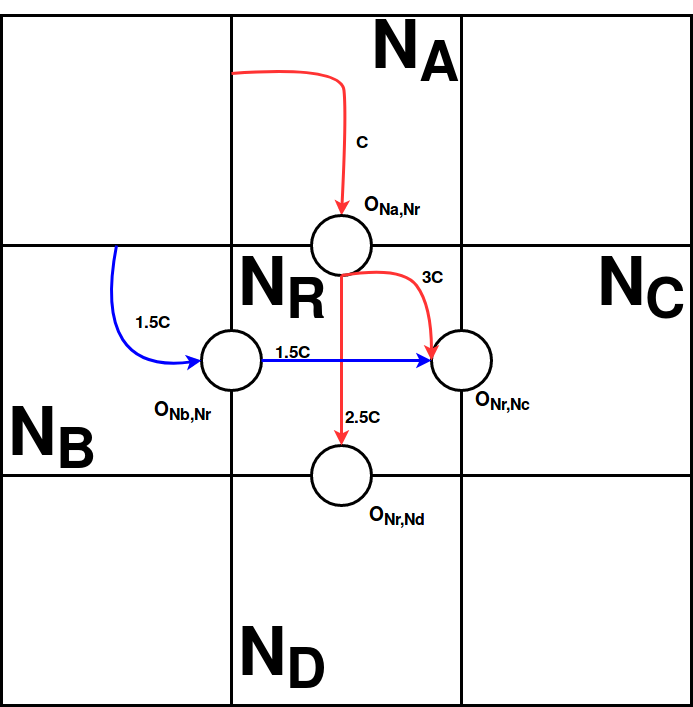
\includegraphics[width=0.6\textwidth]{LookaheadProblem}
\caption{A visual reference for the explanation of the lookahead problem in section 4.3}
\label{LookaheadRef}
\end{figure}
